% ---------------------------------------------------------------------------
% Esquemático de cableado del arnés de loopback RS485 a dos hilos, entre dos
% conectores D-Sub-9, usado para verificar comunicaciones RS485.
% Fuente del PDF que incluye la memoria (capítulo 3).
%
% Compilar:  pdflatex diagrama_arnes_loopback.tex
% ---------------------------------------------------------------------------
\documentclass[border=8pt]{standalone}
\usepackage[utf8]{inputenc}
\usepackage[T1]{fontenc}
\usepackage{lmodern}
\usepackage{tikz}
\usetikzlibrary{arrows.meta, calc}

\definecolor{cPropio}{HTML}{2A78D6}   % azul: diseño propio de la placa
\definecolor{cIP}{HTML}{EDA100}       % ámbar: circuito integrado de terceros
\definecolor{cExt}{HTML}{1BAF7A}      % aguamarina: fuera de la placa
\definecolor{cRef}{HTML}{8A8A85}      % gris: líneas, bandas y contornos

\begin{document}
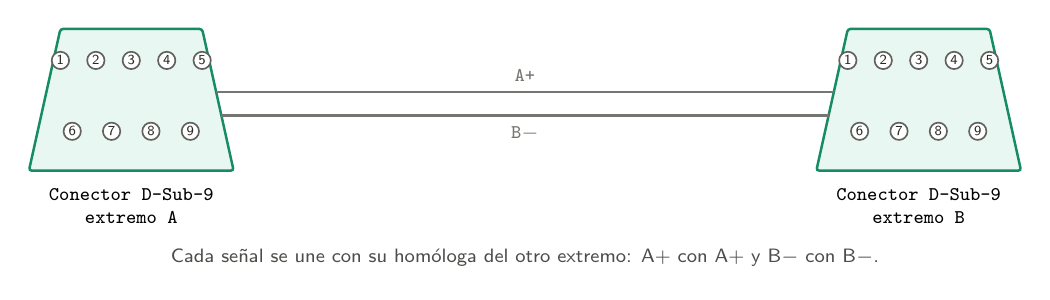
\begin{tikzpicture}[
    x=1cm, y=1cm, font=\sffamily\small,
    ext/.style={draw=cExt!80!black, line width=0.9pt, rounded corners=1pt,
                fill=cExt!10},
    pin/.style={draw=cRef!70!black, line width=0.6pt, fill=white},
    pinnum/.style={font=\tiny\sffamily, text=cRef!30!black},
    wire/.style={draw=cRef!85!black, line width=1pt},
    lbl/.style={font=\sffamily\scriptsize, inner sep=2pt},
    tlbl/.style={font=\ttfamily\scriptsize, inner sep=2pt},
    name/.style={font=\ttfamily\scriptsize, align=center},
]

% ===================== Conector A (izquierda) =====================
\draw[ext] (2.6-1.3,0) -- (2.6+1.3,0) -- (2.6+0.9,1.8) -- (2.6-0.9,1.8) -- cycle;
\foreach \i/\dx in {1/-0.9,2/-0.45,3/0,4/0.45,5/0.9}{
    \draw[pin] (2.6+\dx,1.4) circle (0.11);
    \node[pinnum] at (2.6+\dx,1.4) {\i};
}
\foreach \i/\dx in {6/-0.75,7/-0.25,8/0.25,9/0.75}{
    \draw[pin] (2.6+\dx,0.5) circle (0.11);
    \node[pinnum] at (2.6+\dx,0.5) {\i};
}
\node[name] at (2.6,-0.45) {Conector D-Sub-9\\extremo A};

% ===================== Conector B (derecha) =====================
\draw[ext] (12.6-1.3,0) -- (12.6+1.3,0) -- (12.6+0.9,1.8) -- (12.6-0.9,1.8) -- cycle;
\foreach \i/\dx in {1/-0.9,2/-0.45,3/0,4/0.45,5/0.9}{
    \draw[pin] (12.6+\dx,1.4) circle (0.11);
    \node[pinnum] at (12.6+\dx,1.4) {\i};
}
\foreach \i/\dx in {6/-0.75,7/-0.25,8/0.25,9/0.75}{
    \draw[pin] (12.6+\dx,0.5) circle (0.11);
    \node[pinnum] at (12.6+\dx,0.5) {\i};
}
\node[name] at (12.6,-0.45) {Conector D-Sub-9\\extremo B};

% ===================== Hilos: A+ y B- =====================
% Los hilos salen del hueco entre las dos filas de contactos porque la
% memoria no especifica a qué pin concreto se conecta cada señal.
\draw[wire] (3.68,1.00) -- (11.52,1.00);
\node[tlbl, anchor=south, text=cRef!85!black] at (7.60,1.06) {A+};

\draw[wire] (3.74,0.70) -- (11.46,0.70);
\node[tlbl, anchor=north, text=cRef!85!black] at (7.60,0.64) {B$-$};

% ===================== Nota =====================
\node[lbl, text=cRef!55!black, align=center] at (7.60,-1.10)
      {Cada señal se une con su homóloga del otro extremo: A+ con A+ y B$-$ con B$-$.};

\end{tikzpicture}
\end{document}
